\documentclass{article}
\usepackage{tikz}
\usepackage{pgfplots}
\pgfplotsset{compat=1.18}

\begin{document}

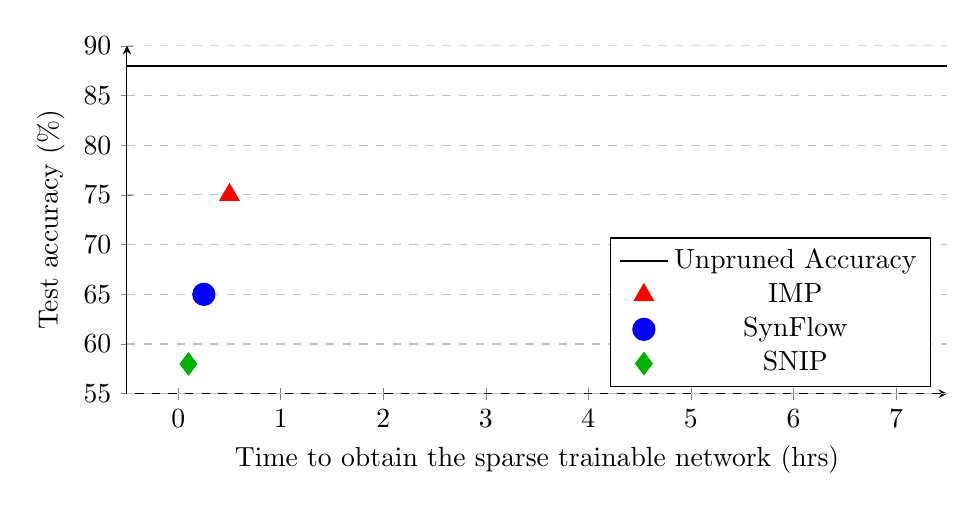
\begin{tikzpicture}
\begin{axis}[
    width=12cm,
    height=6cm,
    xlabel={Time to obtain the sparse trainable network (hrs)},
    ylabel={Test accuracy (\%)},
    xmin=-0.5, xmax=7.5,
    ymin=55, ymax=90,
    ytick={55,60,65,70,75,80,85,90},
    xtick={0,1,2,3,4,5,6,7},
    ymajorgrids=true,
    grid style={dashed, gray!30},
    legend style={at={(0.98,0.02)}, anchor=south east},
    axis lines=left,
]

% Horizontal line for unpruned accuracy
\addplot[
    thick,
    black,
] coordinates {
    (-0.5,88)
    (7.5,88)
};
\addlegendentry{Unpruned Accuracy}

% Data points for different methods
\addplot[
    only marks,
    mark=triangle*,
    mark size=4pt,
    red,
] coordinates {
    (0.5,75)
};
\addlegendentry{IMP}

\addplot[
    only marks,
    mark=*,
    mark size=4pt,
    blue,
] coordinates {
    (0.25,65)
};
\addlegendentry{SynFlow}

\addplot[
    only marks,
    mark=diamond*,
    mark size=4pt,
    green!70!black,
] coordinates {
    (0.1,58)
};
\addlegendentry{SNIP}

% Add horizontal dashed lines for better readability
\draw[dashed, gray!50] (axis cs:-0.5,85) -- (axis cs:7.5,85);
\draw[dashed, gray!50] (axis cs:-0.5,80) -- (axis cs:7.5,80);
\draw[dashed, gray!50] (axis cs:-0.5,75) -- (axis cs:7.5,75);
\draw[dashed, gray!50] (axis cs:-0.5,70) -- (axis cs:7.5,70);
\draw[dashed, gray!50] (axis cs:-0.5,65) -- (axis cs:7.5,65);
\draw[dashed, gray!50] (axis cs:-0.5,60) -- (axis cs:7.5,60);
\draw[dashed, gray!50] (axis cs:-0.5,55) -- (axis cs:7.5,55);

\end{axis}
\end{tikzpicture}

\end{document}